\documentclass[20pt,margin=1in,innermargin=-4.5in,blockverticalspace=-0.25in]{tikzposter}
\geometry{paperwidth=42in,paperheight=32.5in}
\usepackage[utf8]{inputenc}
\usepackage{amsmath}
\usepackage{amsfonts}
\usepackage{amsthm}
\usepackage{amssymb}
\usepackage{mathrsfs}
\usepackage{graphicx}
\usepackage{adjustbox}
\usepackage{enumitem}
\usepackage[backend=biber,style=numeric]{biblatex}
\usepackage{UWtheme}
\usepackage{svg}
\usepackage{caption}

\usepackage{mwe} % for placeholder images

% set theme parameters
\tikzposterlatexaffectionproofoff
\usetheme{UWTheme}
\usecolorstyle{UWStyle}

\usepackage[scaled]{helvet}
\renewcommand\familydefault{\sfdefault} 
\usepackage[T1]{fontenc}


\title{Phonon Broadening in InP Solar Cells}
\author{Johannes Byle, Ian Sellers, Collin Brown, Vincent R. Whiteside}
\institute{University of Oklahoma - Photovoltaic Materials and Devices Group}
\titlegraphic{\includegraphics[width=0.25\textwidth]{test.png}}

% begin document
\begin{document}
\maketitle
\centering
\begin{columns}
    \column{0.32}
    \block{Background}{
         Thermalization losses are the one of the largest sources of energy loss in solar cells. These losses occur when photons excite an electron to an energy level above the band gap of the material. When these electrons fall back down to the conduction band of the material they release energy by creating lattice vibrations. The quasiparticle describing these lattice vibrations is called a phonon. Combining different materials and creating materials with quantum structures such as quantum dots or wells has the potential to limit or change these phonon interactions. Understanding how these materials affect phonon interactions could thus make it possible to create solar cells with greatly increased efficiency. 
        \begin{tikzfigure}[\normalsize{Energy losses of an ideal silicon solar cell under the solar spectrum on earth.\cite{1}}]
            \includegraphics[width=0.9\linewidth]{Spectrum.jpg}
        \end{tikzfigure}
    }
    \block{Experimental}{
         It is possible to study phonons using methods such as photoluminescence (PL) and photoreflectance (PR) spectroscopy. Photoluminescence spectroscopy measures the amount of light emitted from a material when it absorbs photons. Photoreflectance spectroscopy measures the change in the reflectivity of a material as its internal dielectric function is modulated by a laser. Photoluminescence is useful for studying phonons because in InP solar cells the temperature dependent change in slope of the high energy tail of the PL spectrum is related to the energy of the phonons in the material.\cite{2}
         \begin{tikzfigure}[\normalsize{One of the experimental setups we tested for taking PR measurements. The solar cell samples are visible in the bottom right corner in the cryostat.}]
             \includegraphics[width=0.9\linewidth]{lab_setup.jpg}
        \end{tikzfigure}
        }
        \column{0.36}
        \block{Analysis}{
         PR spectroscopy is useful because the PL spectrum has several factors affecting the slope of the high energy tail such as impurities and phonon broadening, as well as other features/peaks in the spectrum. The contribution of impurities and phonon broadening must be taken into account in order to extract the correct phonon energy from the PL data. These factors are related to the broadening ($\Gamma_{Tot}$, the full width of the PL peak at half of the maximum of the peak) of the low energy side of the PL spectrum according to the following equation.\cite{2}
         \begin{equation}
         \Gamma_{Tot}\left(T\right)=\Gamma_0+\Gamma_{LA}T+\frac{\Gamma_{LO}}{\left[\exp\left(\frac{h\omega_{LO}}{k_BT}\right)\right]}+\Gamma_{Imp}\exp\left(-\frac{E_B}{k_BT_H}\right)
         \end{equation}
        \begin{tikzfigure}[\normalsize{InP solar cell PL spectra at different temperatures.}]
             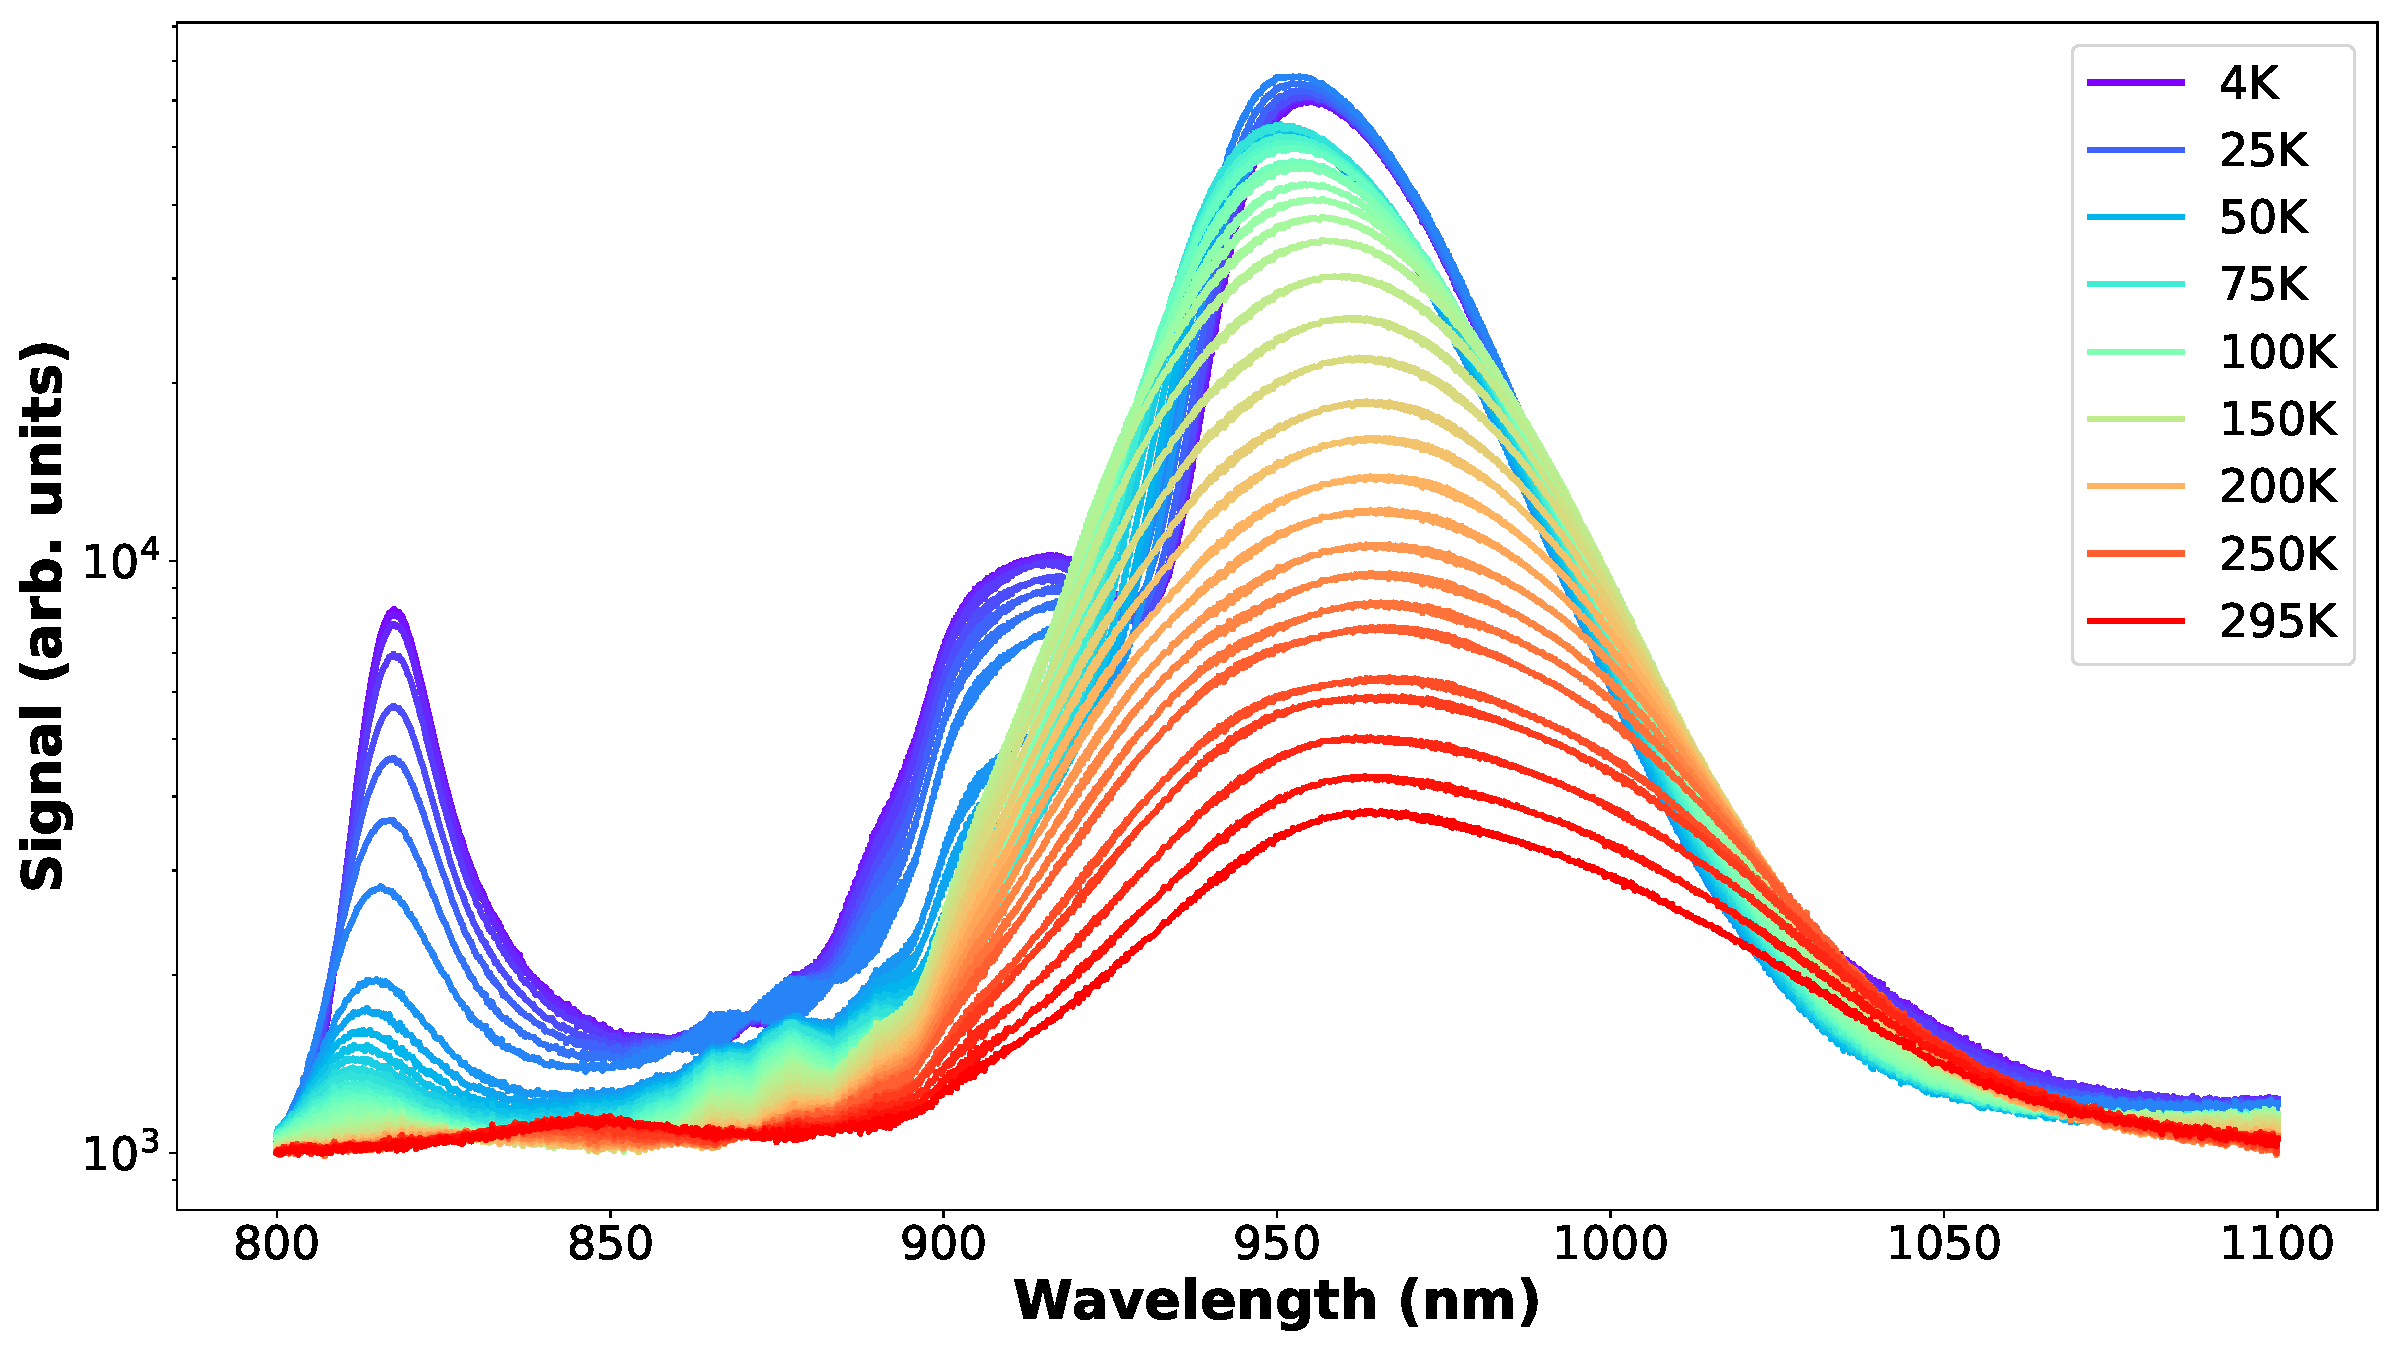
\includegraphics[width=0.9\linewidth]{InP_SQW.pdf}
        \end{tikzfigure}
        One of the factors that needs to be taken into account in order to extract the correct phonon energy is the optical phonon broadening $\Gamma_{LO}$. The phonon broadening can be estimated from the PL data, but it can also be extracted from the PR data by fitting the PR data to following equation which describes how the normalized change in reflectance is related to the band gap and broadening of the material.\cite{3}
        \begin{equation}
        \frac{\Delta R}{R}=\Re\left[Ae^{i\gamma}(E-E_g+i\Gamma)^{-m}\right]
        \end{equation}
        \begin{tikzfigure}[\normalsize{PR spectra of GaAs at different temperatures.}]
             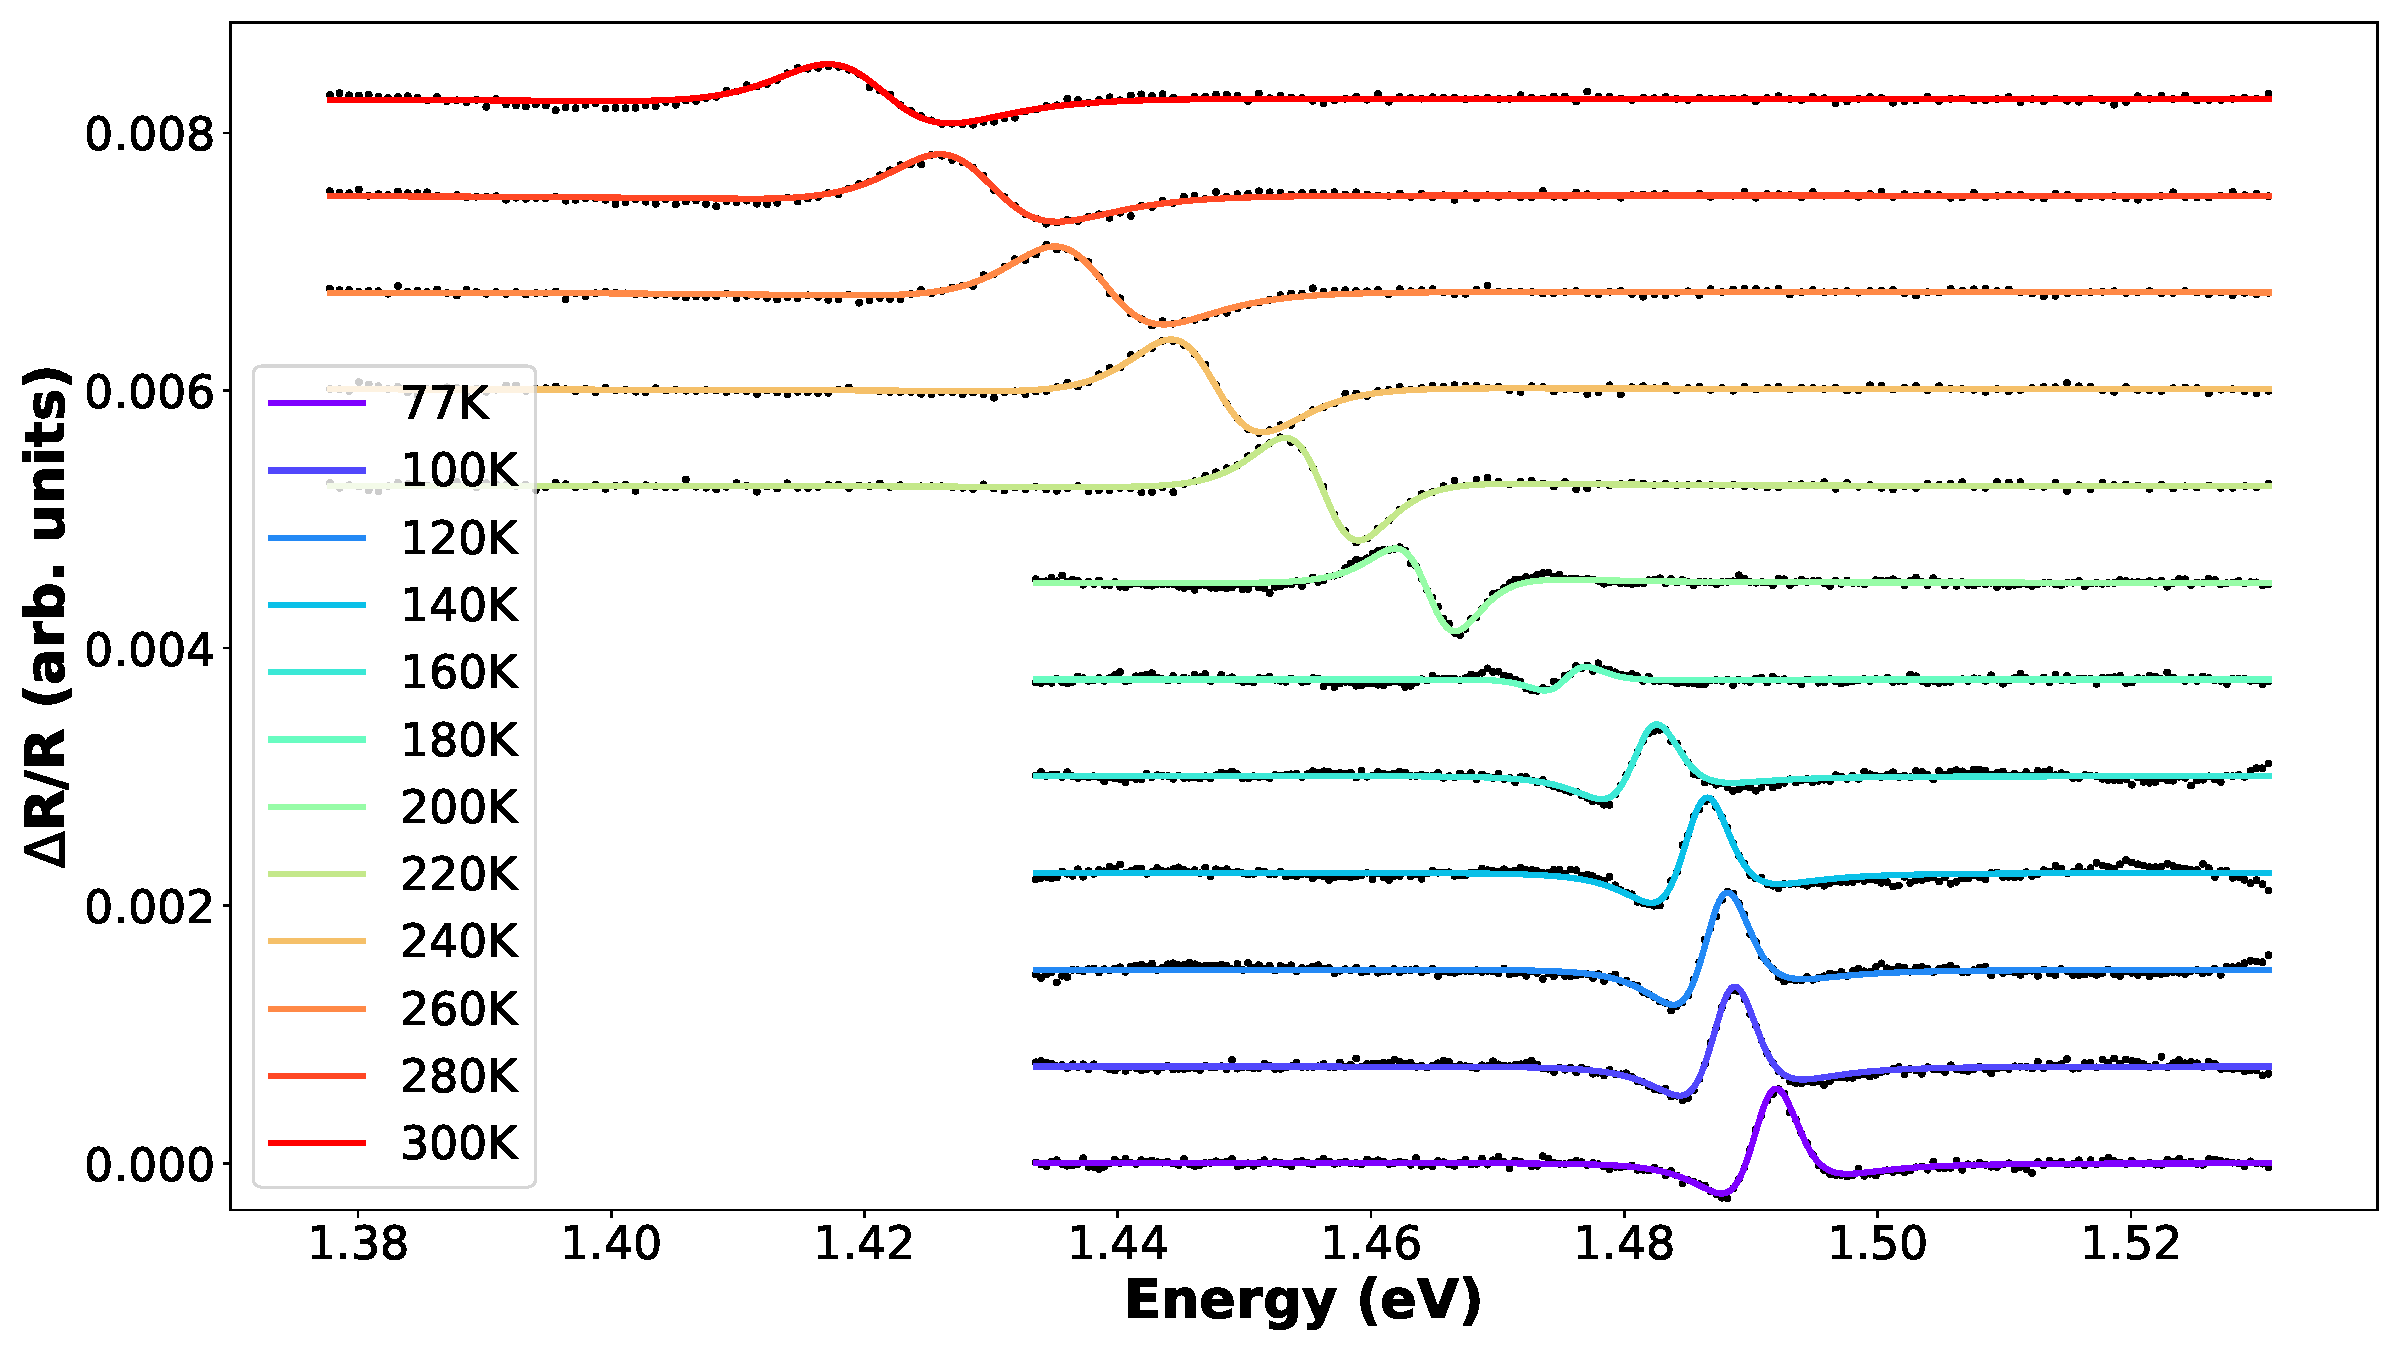
\includegraphics[width=0.9\linewidth]{GaAs.pdf}
        \end{tikzfigure}
         }f

    \column{0.32}
    \block{Conclusion}{
    
       We successfully extracted the phonon broadening factors from the InP PL data using equation 1.
        \begin{tikzfigure}[\normalsize{Broadening $\Gamma_{Tot}$ of the InP PL data vs temperature.}]
            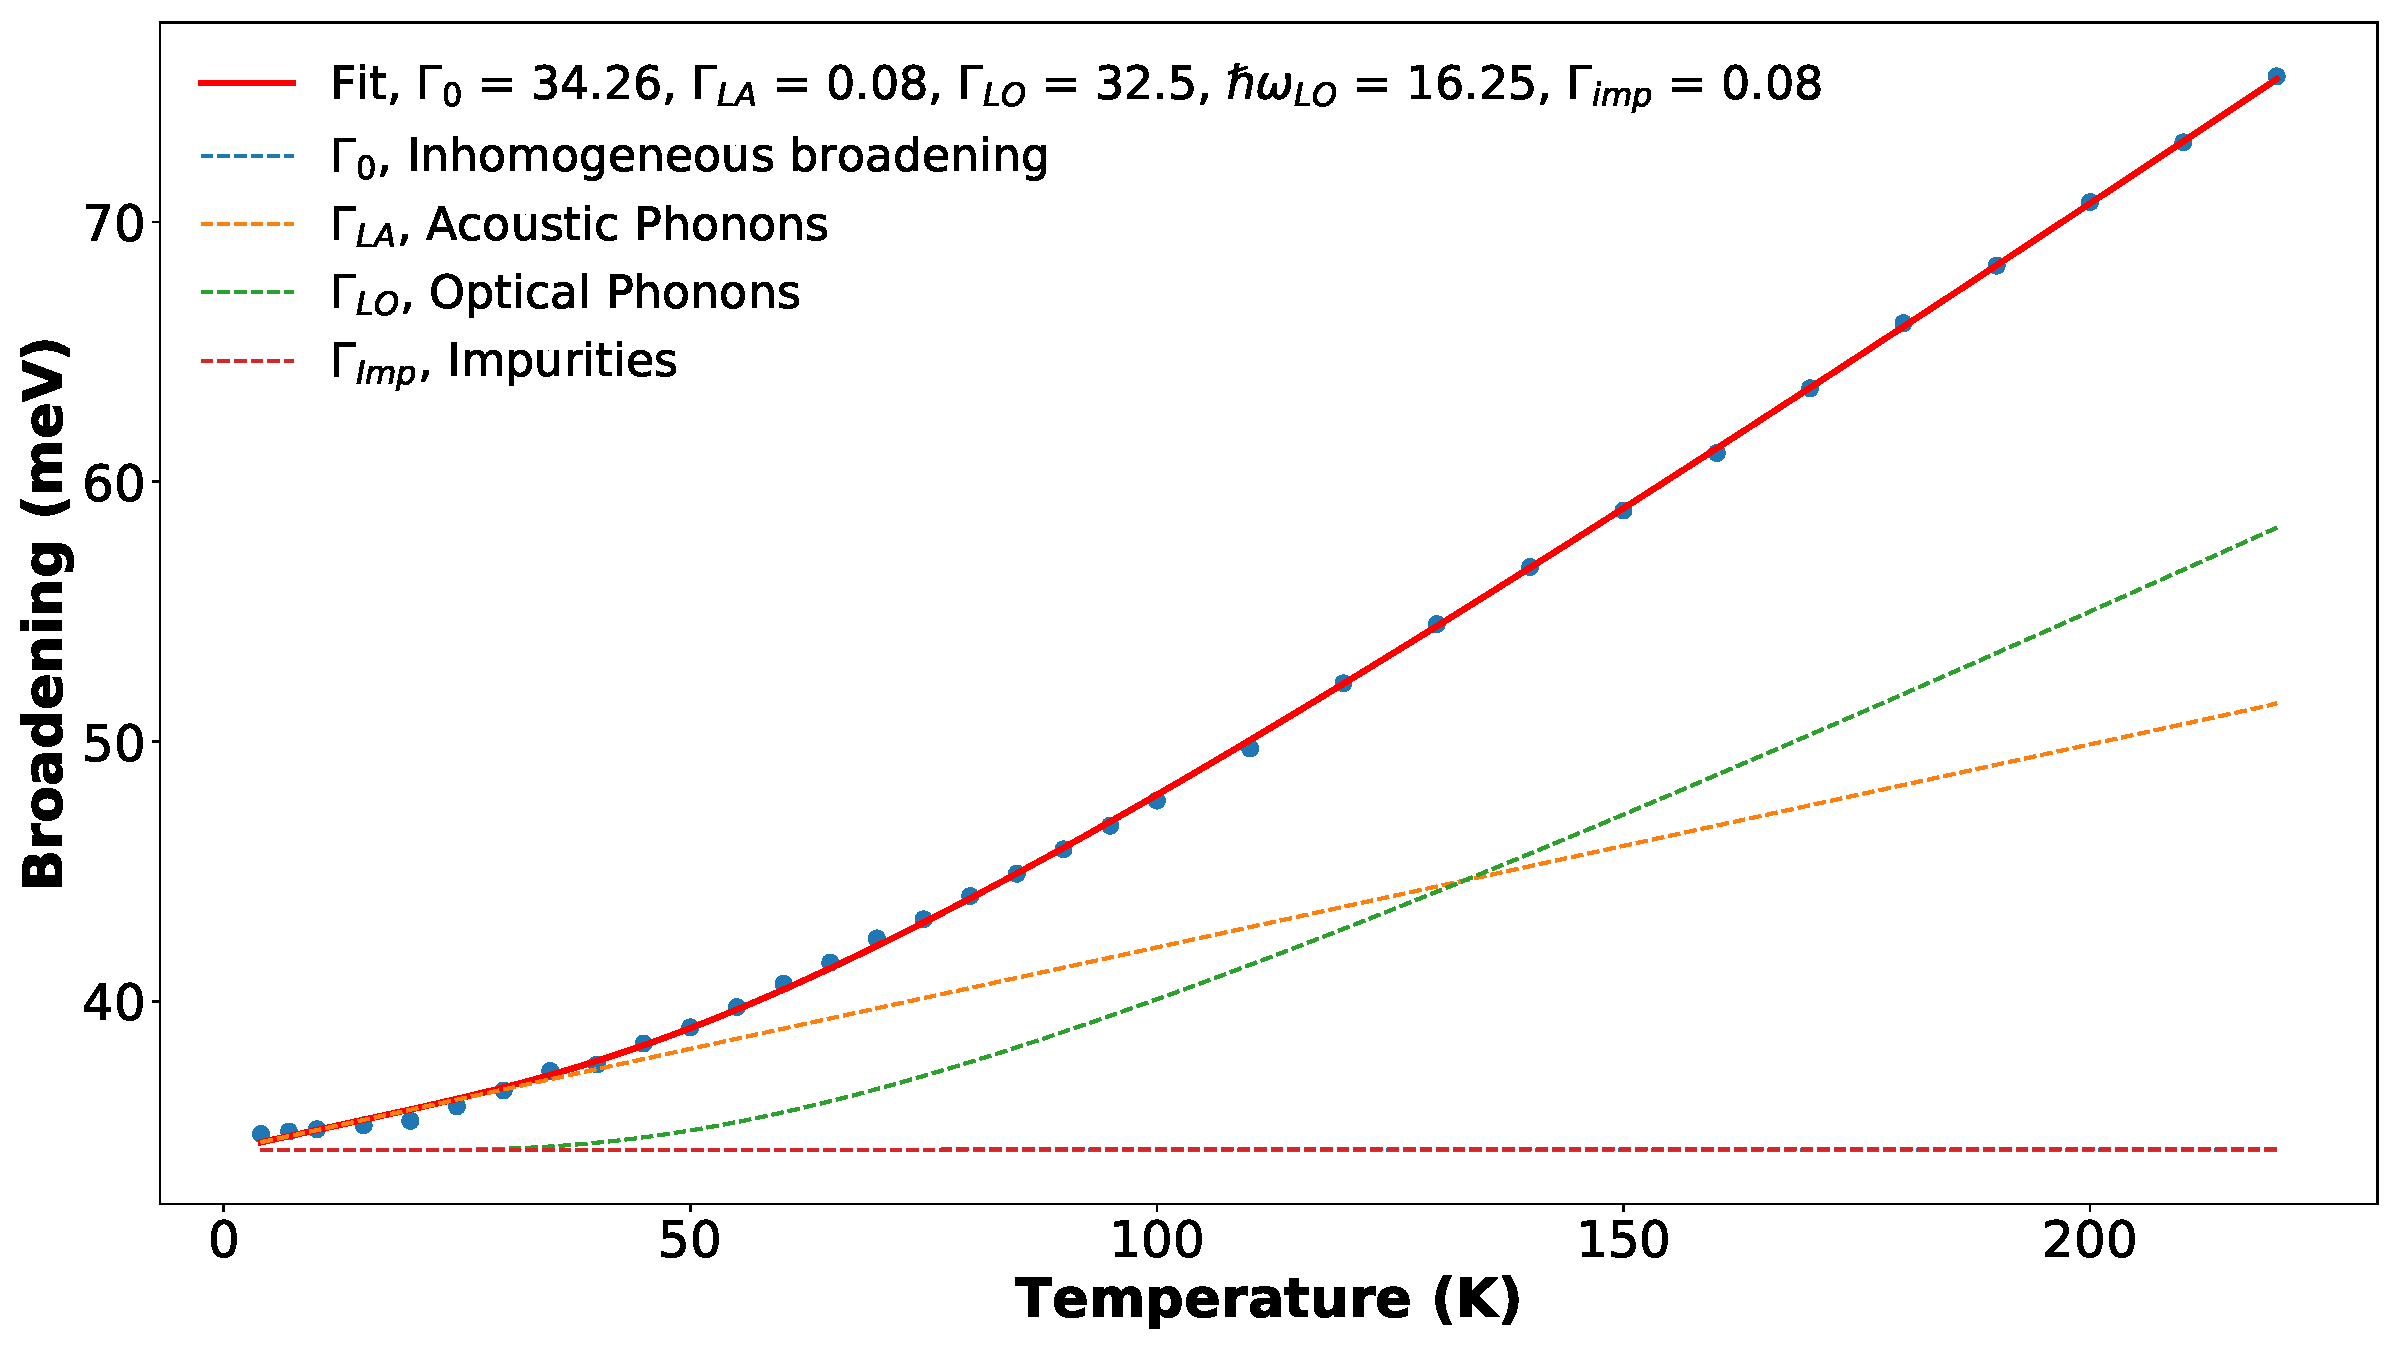
\includegraphics[width=0.9\linewidth]{fit.pdf}
        \end{tikzfigure}
        Although we were not able to improve the experimental setup enough to take PR measurements of the InP solar cells, we created code to extract fitting factors from PR data and were able to confirm the accuracy of our GaAs PR measurements.
                \begin{tikzfigure}[\normalsize{Change in band gap energy of GaAs (blue) and the value predicted by the Bose-Einstein equation (red).}]
            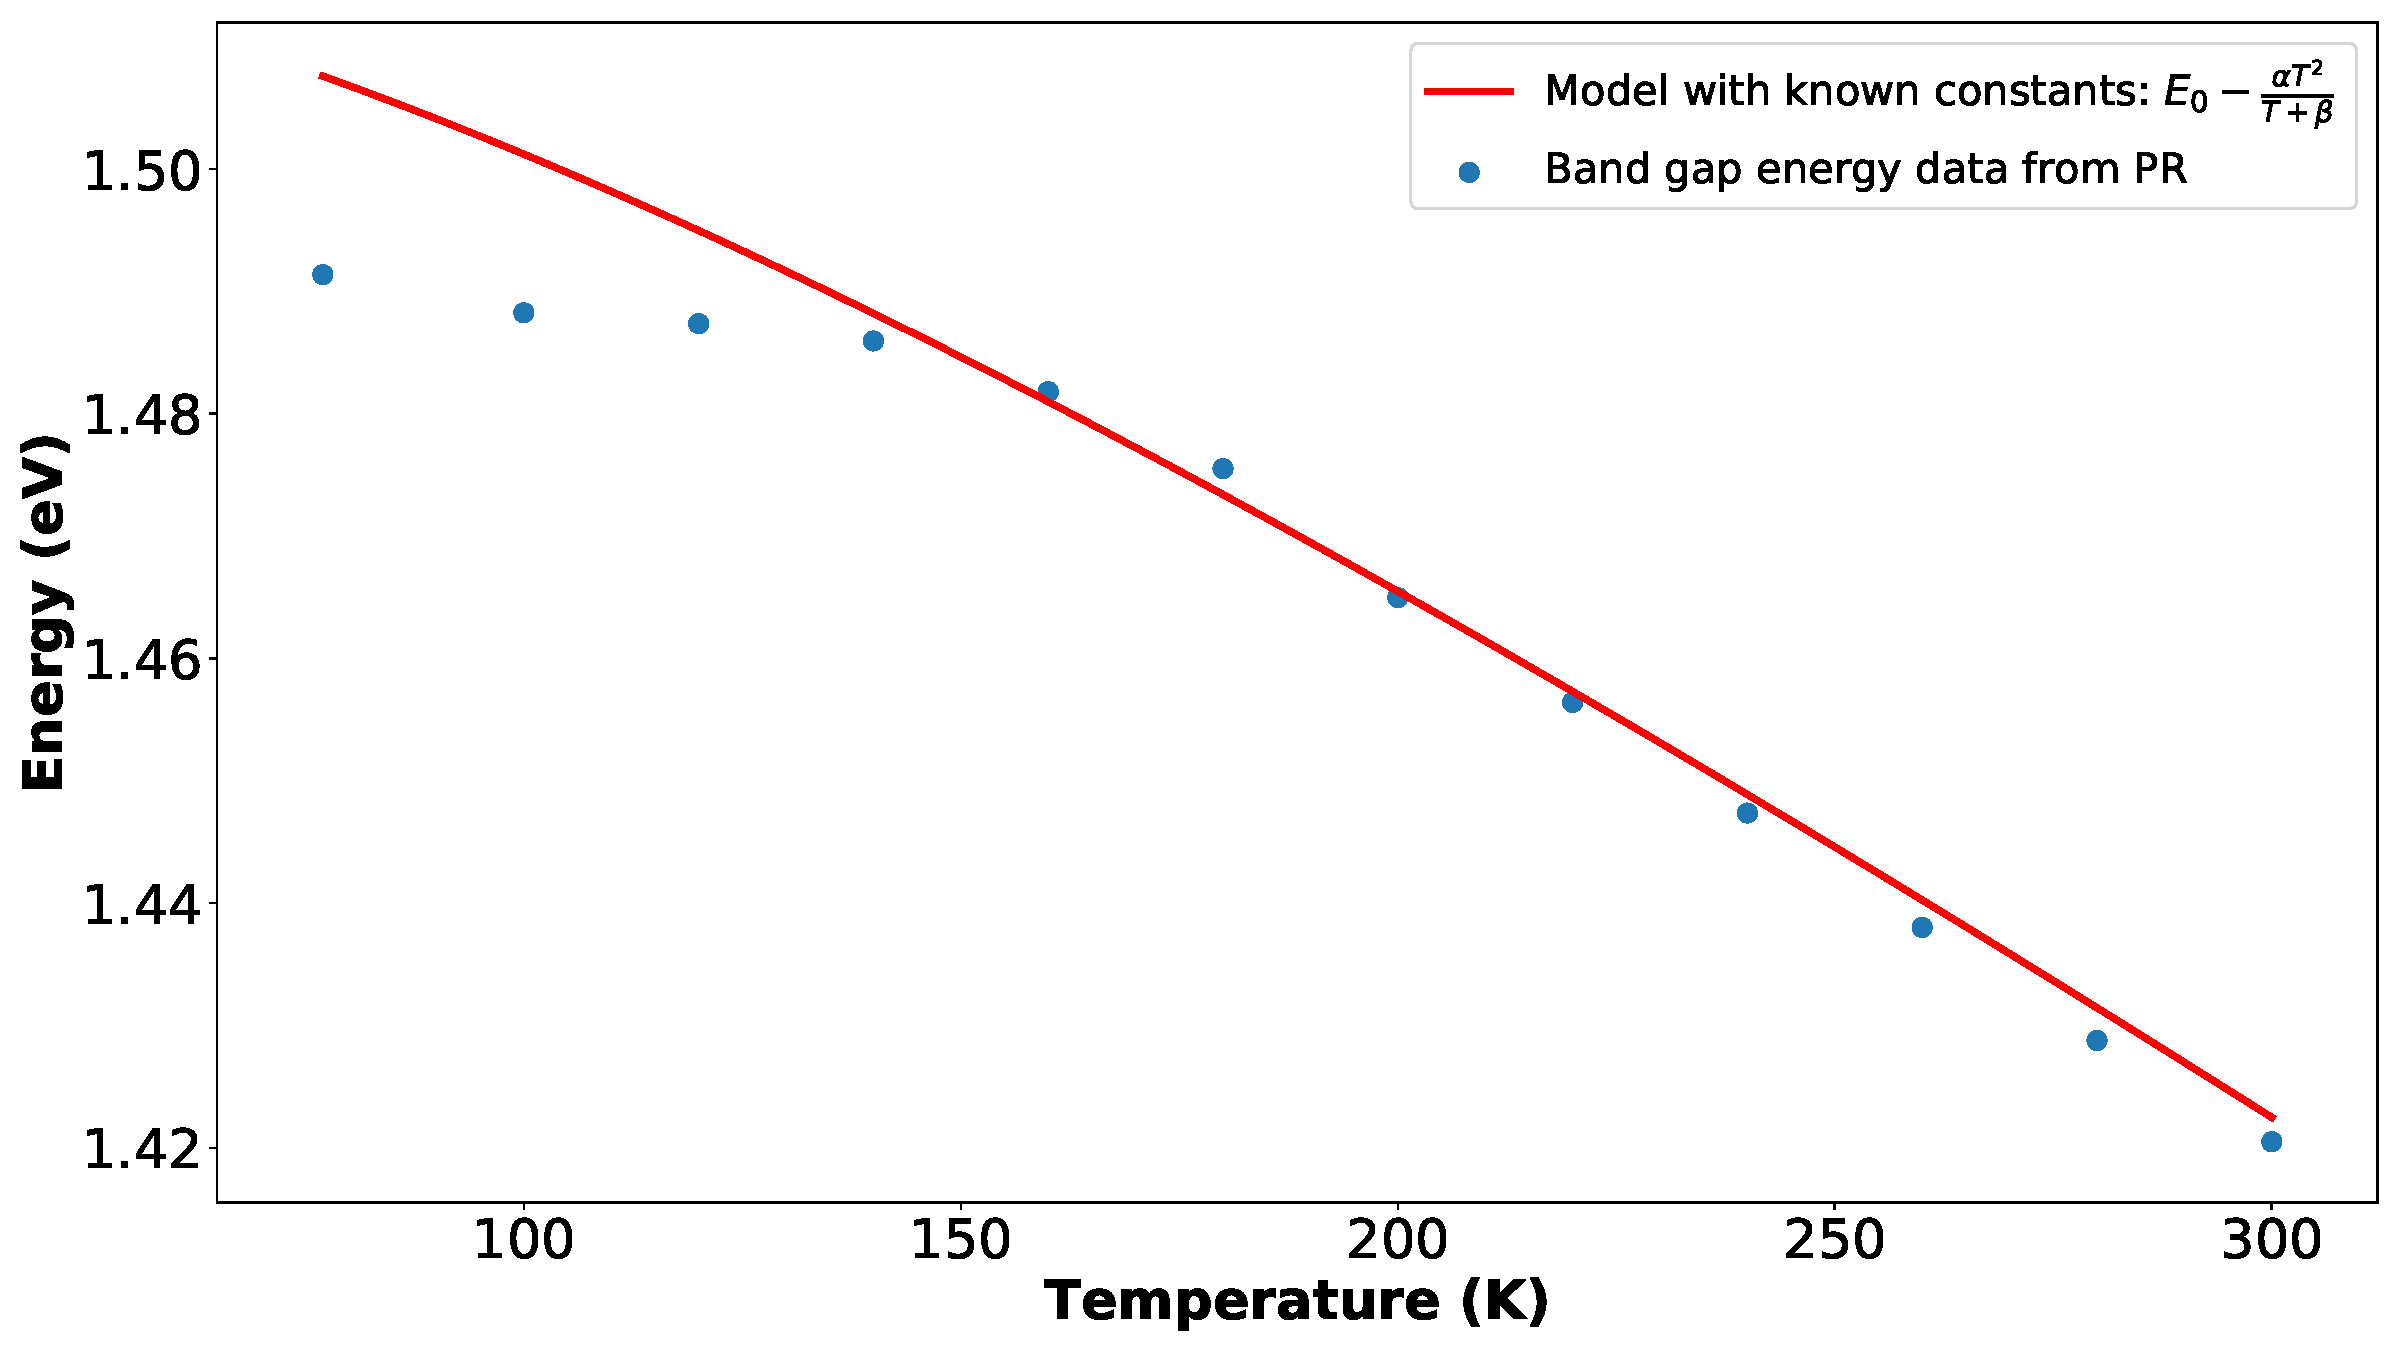
\includegraphics[width=0.9\linewidth]{GaAs_fit.pdf}
        \end{tikzfigure}
    }


    
    \block{References}{
        \vspace{-1em}
        \begin{footnotesize}
        \begingroup
		\renewcommand{\section}[2]{}%
        \begin{thebibliography}{}
 
\bibitem{Octavi} 
Octavi E. Semonin, Joseph M. Luther, Matthew C. Beard
\textit{Quantum dots for next-generation photovoltaics}. 
Materials Today, Volume 15, Issue 11, 2012, Pages 508-515

\bibitem{Sellers} 
Hamidreza Esmaielpour Vincent R. Whiteside Louise C. Hirst Joseph G. Tischler Chase T. Ellis Matthew P. Lumb David V. Forbes Robert J. Walters Ian R. Sellers
\textit{Effect of occupation of the excited states and phonon broadening on the determination of the hot carrier temperature from continuous wave photoluminescence in InGaAsP quantum well absorbers}. 
Prog. Photovolt: Res. Appl. Volume 25, Issue 9, 2017

\bibitem{Aspnes}
Jan Misiewicz, Piotr Sitarek, Grzegorz Sek, Robert Kudrawuiec
\textit{Semiconductor heterostructures and device structures investigated by photoreflectance spectroscopy}. 
Materials Science, Vol. 21, No. 3, 2003
\end{thebibliography}
\endgroup
        \end{footnotesize}
    }
    \block{Acknowledgments}{
    This REU research was supported by the National Science Foundation (NSF).
    }
\end{columns}
\end{document}